\chapter{Results and Discussion}
\label{chap:evaluation}
We have already looked at the details of IaaS and how it works technically.
Now it's time to give you some insights how such cloud infrastructures are implemented in real life and how resources can be provided and used by the consumers. Therefore we want to illustrate some concrete representatives who are are operating as a successful IaaS provider in practice in the following chapter.

\section{Amazon Elastic Compute Cloud (Amazon EC2)}

\subsection{A first glance on Amazon's world}
Amazon EC2 is part of the big Cloud Platform of the famous and globally well-known internet company Amazon.com, Inc., namely Amazon Web Services (AWS). AWS started offering IT infrastructure services to businesses using this Cloud computing model already in 2006. Today it's probably the most popular representative in this kind of IT sector offering highly reliable, scalable and low-cost infrastructure platform in the cloud used by a huge number of businesses in currently 190 countries around the world. They emphasize and try to implement the several benefits Cloud computing brings with it. Consumers should avoid hight initial costs to get their infrastructure running, instead a variable cost model with a pay-as-you-go price model should make their work much more cost-effective. Furthermore setting up and maintaining infrastructure components should not be a common task businesses should care about. In contrast the focus should be set on the major issues regarding the concrete business and infrastructure capacity can be provided by AWS with just a click on-demand. AWS truly offers a broad variety of several different services distinguished by it's provided resource type. A typical key benefit someone often face when talking about and using AWS is the perfect interoperability of all the platform components comprising it. That's probably a major point what makes AWS so beloved by customers around the globe. Next to storage(Amazon S3) or networking (Amazon VPC) compute resources, managed by Amazon EC2 are essential to every business as these are the physical machines services need to be alive. [3]

\subsection{EC2 Insights}
Amazon EC2 is designed for web and system administrators to make their lives easier. It provides easy manageable compute capacity available in the cloud. Via a web interface the administrator can request more or less capacity with just a few clicks within minutes. Some more minutes later the required instances are fully set-up with the desires of the user and ready-to-go. This allows the user to scale up and down (which means renting more or compute capacity) on the fly depending on the current demand and without any need to configure them manually. To give this explanation further importance and motivate why Amazon EC2 is the right choice for so many businesses, we want to look at some key benefits this cloud technology introduces in contrast to buying just traditional dedicated hardware at the provider of your trust. 

\subsubsection{Elastic scaling}
As already mentioned the customer can add and remove EC2 instances as she likes and therefore adapt the available compute capacity based on the current demand. It doesn't matter whether someone commissions just a few or even thousands of instances simultaneously. [3] Especially for companies whose resource demand is highly unpredictable due to the reason that they can't give a good guess about the future development of their product this EC2 technology can help them a lot. A question which probably arises is what happens if workload on the EC2 instances varies heavily due to the nature of the application. For instance there could be the case that load heavily depends on some special days or time and always manually enlarging and shrinking the cloud infrastructure would be again an overhead. For this reasons Amazon introduced the Auto Scaling feature where the capacity dynamically scales up and down depending on the current resource demand. The user has opportunities to define peaks and troughs or specific time points where EC2 should react with scaling. So on the one hand you can ensure that there is always enough capacity to deal with the current load and on the other hand you can minimize your costs as you don't waste money for capacity you don't even need at the moment. Over the years Amazon developed some further possibilities for customers to get the most "bang for the buck". With the so called Reserved Instances they established a model where customers can agree to select one of the predefined instance types, pay some low initial costs for each instance they want to reserve and get a significant discount in variable costs. If you are not satisfied with your instances anymore you still have the possibility to place them in another AWS region, change the instance type or even sell capacity to other projects that end before the time frame for the Reserved instances expires. A further pretty nice instance model are Amazon EC2 Spot instances. With Spot instances the user can bid on the hourly price per instance she want to spend. Compute capacity again increases and decreases dynamically and as long as the bid meets or exceeds the instance price which customers commit to pay they gain access to them. This is a great possibility to be sure not to pay more than you actually want and prevent the risk that you oversee massive scaling. [3]

\subsubsection{Elastic Load Balancing (ELB)}
ELB is an intelligent solution to improve both scalability and fault tolerance. The load balancer component automatically distributes incoming traffic throughout the available instances to balance the load equally. It seamlessly integrates with the Auto Scaling feature described in the section above. You can still set your Auto Scaling conditions and if they are met instances get added to your Auto Scaling Group. This also works fine behind an Elastic Load Balancer. Achieving better fault tolerance is the second core point of using ELB. The Amazon load balancer automatically detects unhealthy instances behind itself and therefore does not distribute any further traffic to them until they get healthy again. So it's basically no problem when one of several instances is down for a while. Amazon lets you spread your EC2 instances within Availability Zones and multiple regions. A region is a specific geographic zone where Amazon operates and contains multiple isolated Availability Zones. Especially for globally operating bigger businesses it is highly recommended to distribute instances throughout several Availability zones and multiple regions as this results in lower latencies and further increases fault tolerance. Although a complete availability zone is offline traffic can be routed to farther away regions intermediately. The nice integration with other Amazon Service such as the new Amazon Route 53 even enables DNS failovers in case the load balancer itself suffers.

\subsubsection{AWS Management Console}
Moreover what makes working with AWS so convenient is how less effort you need to complete such tasks. The AWS Management Console does not require much expertise in system or server administration as it comes with a comfortable graphical user interface along. There you can choose which of the dozens of services you would like to look at and also have root access to any of your EC2 instances and so you can start, stop, check and manage them as you like.  
\begin{figure}[t]
	\centering
		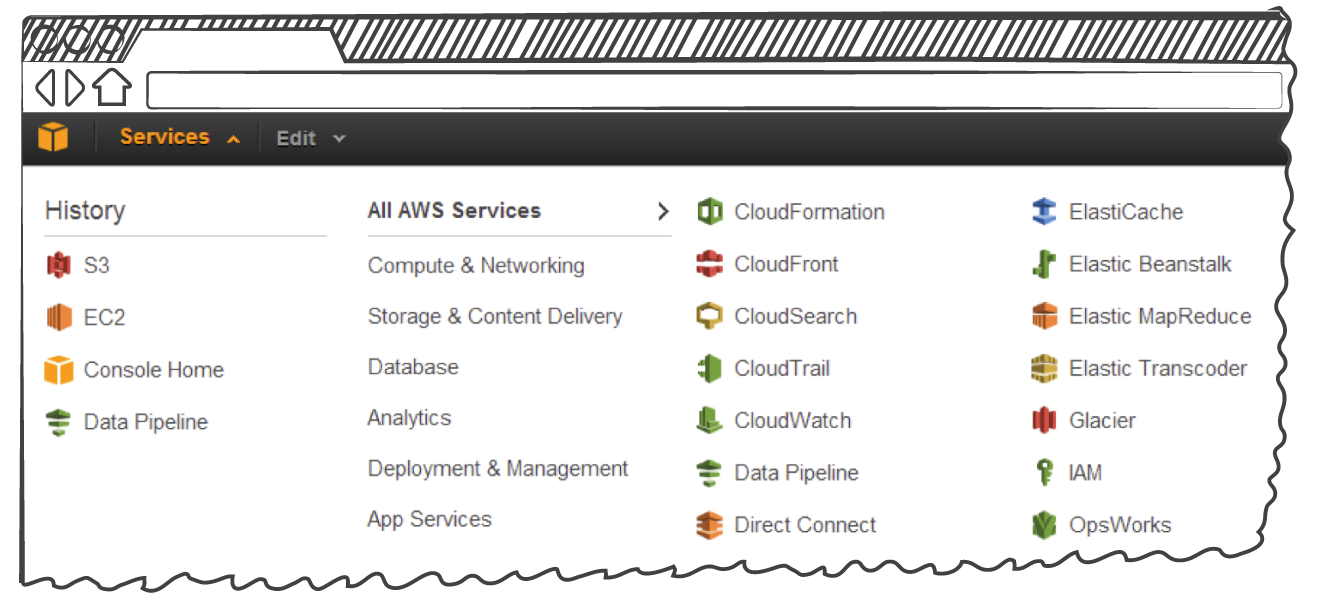
\includegraphics[width=0.90\textwidth]{console_snippet}
	\caption{AWS Management Console - Main overview}
\end{figure}